% Options for packages loaded elsewhere
\PassOptionsToPackage{unicode}{hyperref}
\PassOptionsToPackage{hyphens}{url}
\PassOptionsToPackage{dvipsnames,svgnames,x11names}{xcolor}
%
\documentclass[
  english,
  a4paper,
]{article}
\usepackage{amsmath,amssymb}
\usepackage{lmodern}
\usepackage{iftex}
\ifPDFTeX
  \usepackage[T1]{fontenc}
  \usepackage[utf8]{inputenc}
  \usepackage{textcomp} % provide euro and other symbols
\else % if luatex or xetex
  \usepackage{unicode-math}
  \defaultfontfeatures{Scale=MatchLowercase}
  \defaultfontfeatures[\rmfamily]{Ligatures=TeX,Scale=1}
\fi
% Use upquote if available, for straight quotes in verbatim environments
\IfFileExists{upquote.sty}{\usepackage{upquote}}{}
\IfFileExists{microtype.sty}{% use microtype if available
  \usepackage[]{microtype}
  \UseMicrotypeSet[protrusion]{basicmath} % disable protrusion for tt fonts
}{}
\makeatletter
\@ifundefined{KOMAClassName}{% if non-KOMA class
  \IfFileExists{parskip.sty}{%
    \usepackage{parskip}
  }{% else
    \setlength{\parindent}{0pt}
    \setlength{\parskip}{6pt plus 2pt minus 1pt}}
}{% if KOMA class
  \KOMAoptions{parskip=half}}
\makeatother
\usepackage{xcolor}
\IfFileExists{xurl.sty}{\usepackage{xurl}}{} % add URL line breaks if available
\IfFileExists{bookmark.sty}{\usepackage{bookmark}}{\usepackage{hyperref}}
\hypersetup{
  pdftitle={Interaction structure constrains the emergence of conventions in group communication},
  pdflang={en},
  colorlinks=true,
  linkcolor={blue},
  filecolor={Maroon},
  citecolor={blue},
  urlcolor={blue},
  pdfcreator={LaTeX via pandoc}}
\urlstyle{same} % disable monospaced font for URLs
\usepackage[margin=25mm]{geometry}
\usepackage{longtable,booktabs,array}
\usepackage{calc} % for calculating minipage widths
% Correct order of tables after \paragraph or \subparagraph
\usepackage{etoolbox}
\makeatletter
\patchcmd\longtable{\par}{\if@noskipsec\mbox{}\fi\par}{}{}
\makeatother
% Allow footnotes in longtable head/foot
\usepackage{footnote} % For some unknown reason, footnotehyper clashes with French
\makesavenoteenv{longtable}
\usepackage{graphicx}
\makeatletter
\def\maxwidth{\ifdim\Gin@nat@width>\linewidth\linewidth\else\Gin@nat@width\fi}
\def\maxheight{\ifdim\Gin@nat@height>\textheight\textheight\else\Gin@nat@height\fi}
\makeatother
% Scale images if necessary, so that they will not overflow the page
% margins by default, and it is still possible to overwrite the defaults
% using explicit options in \includegraphics[width, height, ...]{}
\setkeys{Gin}{width=\maxwidth,height=\maxheight,keepaspectratio}
% Set default figure placement to htbp
\makeatletter
\def\fps@figure{htbp}
\makeatother
\setlength{\emergencystretch}{3em} % prevent overfull lines
\providecommand{\tightlist}{%
  \setlength{\itemsep}{0pt}\setlength{\parskip}{0pt}}
\setcounter{secnumdepth}{-\maxdimen} % remove section numbering
\newlength{\cslhangindent}
\setlength{\cslhangindent}{1.5em}
\newlength{\csllabelwidth}
\setlength{\csllabelwidth}{3em}
\newlength{\cslentryspacingunit} % times entry-spacing
\setlength{\cslentryspacingunit}{\parskip}
\newenvironment{CSLReferences}[2] % #1 hanging-ident, #2 entry spacing
 {% dont indent paragraphs
  \setlength{\parindent}{0pt}
  % turn on hanging indent if param 1 is 1
  \ifodd #1
  \let\oldpar\par
  \def\par{\hangindent=\cslhangindent\oldpar}
  \fi
  % set entry spacing
  \setlength{\parskip}{#2\cslentryspacingunit}
 }%
 {}
\usepackage{calc}
\newcommand{\CSLBlock}[1]{#1\hfill\break}
\newcommand{\CSLLeftMargin}[1]{\parbox[t]{\csllabelwidth}{#1}}
\newcommand{\CSLRightInline}[1]{\parbox[t]{\linewidth - \csllabelwidth}{#1}\break}
\newcommand{\CSLIndent}[1]{\hspace{\cslhangindent}#1}

%%%%%%%% START HEADER PARTIAL %%%%%%%%%%%%

% Formatting of tables & knitr::kable and kableExtra functionality
\usepackage{float}
\usepackage{colortbl}
\usepackage{pdflscape}
\usepackage{tabu}
\usepackage{threeparttable}

% Line numbering

% endfloat stuff

% fancyhdr pagestyle

% Environment for keywords
\makeatletter
\newcommand\keywordsname{Keywords}
\newenvironment*{keywords}[1][\keywordsname]{\if@twocolumn \else \small \quotation \fi \begin{center} \textbf{\textit{#1} \\}}{\end{center}\if@twocolumn \else \small \endquotation \fi}
\newenvironment*{keywordsinline}[1][\keywordsname]{\if@twocolumn \else \small \quotation \fi \begin{center} \textbf{\textit{#1}: }}{\end{center}\if@twocolumn \else \small \endquotation \fi}
\makeatother

% Environment for abstract that takes new abstract name
\newenvironment{renameableabstract}[1][\abstractname]{\let\oldabstractname\abstractname \renewcommand{\abstractname}{#1} \begin{abstract}}{\end{abstract} \renewcommand{\abstractname}{\oldabstractname}}

%%%%%%%% END HEADER PARTIAL %%%%%%%%%%%%

\usepackage{tikz}
\usetikzlibrary{angles,positioning,arrows.meta, quotes, shapes, shapes.geometric}
\usepackage{graphicx}
\usepackage{booktabs}
\usepackage{longtable}
\usepackage{array}
\usepackage{multirow}
\usepackage{wrapfig}
\usepackage{float}
\usepackage{colortbl}
\usepackage{pdflscape}
\usepackage{tabu}
\usepackage{threeparttable}
\usepackage{threeparttablex}
\usepackage[normalem]{ulem}
\usepackage{makecell}
\usepackage{xcolor}
\ifXeTeX
  % Load polyglossia as late as possible: uses bidi with RTL langages (e.g. Hebrew, Arabic)
  \usepackage{polyglossia}
  \setmainlanguage[]{}
\else
  \usepackage[english,main=english]{babel}
% get rid of language-specific shorthands (see #6817):
\let\LanguageShortHands\languageshorthands
\def\languageshorthands#1{}
\fi
\ifLuaTeX
  \usepackage{selnolig}  % disable illegal ligatures
\fi

\title{Interaction structure constrains the emergence of conventions in group communication}

%%%%%%% START AUTHOR PARTIAL %%%%%%%%%%%%%%%

%%%%% Authors, affiliations and author notes stuff %%%%%

% Macros for creating and referencing stored reference
\makeatletter
\def\MyNewLabel#1#2#3{\expandafter\gdef\csname #1@#2\endcsname{#3}}

\def\MyRef#1#2{\@ifundefined{#1@#2}{???}{\csname #1@#2\endcsname}}

\newcommand*\ifcounter[1]{%
  \ifcsname c@#1\endcsname
    \expandafter\@firstoftwo
  \else
    \expandafter\@secondoftwo
  \fi
}
\makeatother

% Create labels for Addresses if the are given by code
\MyNewLabel{ADDRTXT}{Stanford}{Stanford University}
\MyNewLabel{ADDRTXT}{Princeton}{Princeton University}

% Create labels for Footnotes if they are given by code
\MyNewLabel{ANOTETXT}{corresp}{Corresponding author. Email: \href{mailto:vboyce@stanford.edu}{\nolinkurl{vboyce@stanford.edu}}}

%%% Special footnotes for addresses and author footnotes
\usepackage{bigfoot}
\DeclareNewFootnote{Addr}[arabic] % Only used for NOT authblk
\DeclareNewFootnote{ANote}[fnsymbol]

%%% Address and author notes as a function of format %%%
 % Use authblk for affiliations %%%%%%%%%%%
\usepackage{authblk}

% Always separate by commas
\renewcommand\Authsep{, }
\renewcommand\Authand{, }
\renewcommand\Authands{, }

% Counter for addresses and footnotes
\newcounter{addrcnt}

% thanks definition that doesnt produce superscript marks
\makeatletter
\newcommand*\createaddrlblbycode[1]{%
  \ifcounter{ADDRLBL@#1}
    {}
    {\refstepcounter{addrcnt}\newcounter{ADDRLBL@#1}\setcounter{ADDRLBL@#1}{\value{addrcnt}}}%
}

\newcommand*\addrlblbycode[1]{\arabic{ADDRLBL@#1}}

\newcommand*\addrbycode[1]{%
  \ifcounter{ADDR@#1}
    {}
    {\newcounter{ADDR@#1}%
     \affil[\addrlblbycode{#1}]{\MyRef{ADDRTXT}{#1}}}%
}

\newcommand*\createanotelblbycode[1]{%
  \ifcounter{ANOTELBL@#1}
    {}
    {\refstepcounter{footnoteANote}\newcounter{ANOTELBL@#1}\setcounter{ANOTELBL@#1}{\value{footnoteANote}}}%
}

\newcommand*\anotelblbycode[1]{\fnsymbol{ANOTELBL@#1}}

\newcommand*\anotebycode[1]{%
  \ifcounter{ANOTE@#1}
    {}
    {\newcounter{ANOTE@#1}%
     \footnotetextANote[\value{ANOTELBL@#1}]{\MyRef{ANOTETXT}{#1}}}%
}
\makeatother


\createaddrlblbycode{Stanford}


\createanotelblbycode{corresp}

\author[%
\addrlblbycode{Stanford}%
,%
$\anotelblbycode{corresp}$%
]{Veronica Boyce}

\addrbycode{Stanford}


\createaddrlblbycode{Princeton}



\author[%
\addrlblbycode{Princeton}%
]{Robert Hawkins}

\addrbycode{Princeton}


\createaddrlblbycode{Stanford}



\author[%
\addrlblbycode{Stanford}%
]{Noah D. Goodman}

\addrbycode{Stanford}


\createaddrlblbycode{Stanford}



\author[%
\addrlblbycode{Stanford}%
]{Michael C. Frank}

\addrbycode{Stanford}


%endif(authblk)

%%%%%%%%% END AUTHOR PARTIAL %%%%%%%%

\date{}

\begin{document}
\maketitle

%%%%%%%%%% START AFTER TITLE PARTIAL %%%%%%%%%%%%%
\anotebycode{corresp}


%%%%%%%%%% END AFTER TITLE PARTIAL %%%%%%%%%%%%%


\begin{otherlanguage}{english}

\begin{abstract}
Group communication is ubiquitous, but it presents some challenges not found in two-person communication, which is the primary focus of the experimental literature. One test case for communication that is is iterated reference games, where the phenomenon of reduction over repeated reference is well-attested in dyadic contexts and could explain how pairs of people can build shared meanings. We extend the repeated reference game paradigm to groups of 2 to 6 people under varied interaction structure constraints across 313 games (1319 participants). Across conditions, reduction and convergence to shared descriptions occurs, but there is a gradient where smaller groups and groups with thicker communication channels show faster and stronger convergence than larger games or groups with thinner communication channels.

\end{abstract}

\end{otherlanguage}

\hypertarget{todos}{%
\section{TODOs}\label{todos}}

Communicating in groups can be challenging. Listeners may have different levels of background knowledge that the rest of the groups may be unaware of. Some interlocuters may interrupt with questions, and others might pipe in to explain their views, collectively leading to everyone talking at once. Multiple conversations threads may split off that need to merge back together for the group to reach agreement. Different people may understand the same speaker as meaning different things, resulting in disagreements and misunderstandings. Disagreements may even escalate to the point where meta-discussion is needed to define terms or struction the conversation differently. We've all been in situations that look like this, where a conversation with half-a-dozen people devolves into chaos and results in inefficient communication. Yet, despite all of these impediments, we often communicate successfully in groups. How?

One key requirement for efficient communication in groups of any size is a shared vocabulary, or shared mappings between linguistic units and objects or concepts (\protect\hyperlink{ref-traum2004}{Traum 2004}, \protect\hyperlink{ref-ginzburg2005}{Ginzburg \& Fernandez 2005}, \protect\hyperlink{ref-branigan2006}{Branigan 2006}). Because reference is a requirement of communcation that can be isolated and tested in experimentally manipulated contexts, it has been a case study for efficient communication more broadly. In many cases, ther are widely shared convention mappings between objects and descriptions that people can rely on, but in other cases, interlocuters must invent ad-hoc reference expressions to communicate about objects without canonical names.

The formation of these new reference expressions is well-studied in dyadic contexts. Clark \& Wilkes-Gibbs (\protect\hyperlink{ref-clarkReferringCollaborativeProcess1986}{1986}) established an experimental method for studying the emergence of new referring expressions that has now become standard (building on \protect\hyperlink{ref-kraussChangesReferencePhrases1964}{Krauss \& Weinheimer 1964}, \protect\hyperlink{ref-kraussConcurrentFeedbackConfirmation1966}{1966}). Two participants see the same set of figures; the speaker describes each figure in turn so the listener can select the target from the set of figures. The speaker and listener repeat this process with the same images over a series of blocks. Early descriptions are long and make reference to multiple features in the figure, but in later iterations, shorthand conventional names for each figure emerge; this shortening of utterances is called `reduction'.

Recently, online participant recruitment and web-based experiments have made it possible to study this convergence in larger populations (\protect\hyperlink{ref-haber2019}{Haber et al. 2019}, \protect\hyperlink{ref-hawkinsCharacterizingDynamicsLearning2020}{Hawkins et al. 2020}). In line with results from face-to-face, oral paradigms, speakers reduced their utterances, producing fewer words per image in later blocks than in earlier blocks. (Throughout this paper, we use ``speaker'' and ``listener'' to refer to the roles describing and selecting targets, regardless of communication modality.)

Dyads are robustly successful at forming conventionalized shorthands in iterated reference games, but talking with one person omits some sources of complexity that are involved with talking to multiple. How does the formation of shared conventions proceed in multi-party communication?

In the current work, we address how components of interaction structure, including group size and communication channels, shape how successfully groups form partner-specific conventionalized names for target objects over the course of an iterated reference game. We recruited 1319 participants who were organized into 313 groups distributed across 3 online experiments and 11 conditions. Collectively, players produced 326000 during their games. We analysed the results using traditional metrics of accuracy and number of words, and we used computation measures of semantic similarity to understand how utterances evolve during the games.

We find that the characteristic pattern of increasing accuracy and decreasing utterance length that is noted in the dyadic literature also occurs across conditions in multi-player games. Reduction is coupled with semantic shifts as utterances converge toward the eventual conventionalized name and away from descriptions used by other groups or for other tangrams. These convention-formation phenomena emerge across disparate conditions; however, there are gradient effects where larger groups and groups with narrower communication channels are less effective and converge more slowly and weakly than other groups.

\begin{figure*}[t!]

{\centering 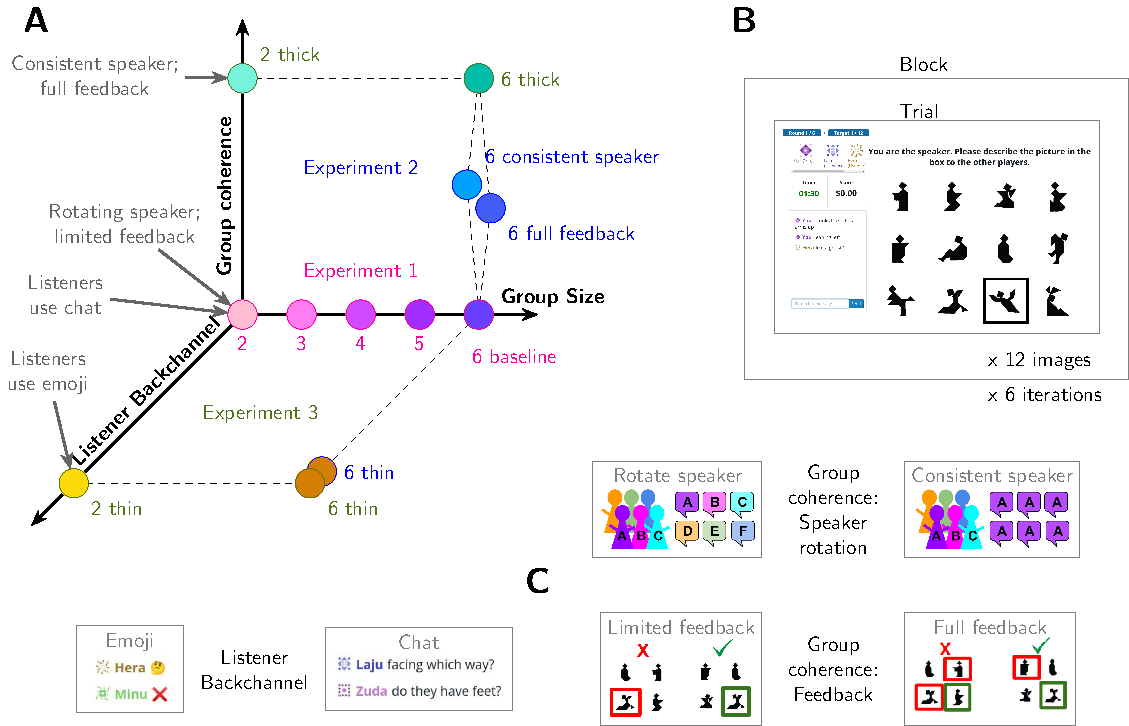
\includegraphics[width=1\linewidth]{expt-diagram} 

}

\caption{TODO: needs some visual help!. \ A: Diagram of the experimental space explored in these experiments. Experiments varied along 3 dimensions: Group size, group coherence, and listener backchannel. Each condition is shown as a dot. Experiment 1 (pink labels) varied group size from 2-6 players while holding group coherence and backchannel constant. Experiment 2 (blue labels) keep group size constant at 6 and varied the other dimensions. Relative to experiment1, 6 single speaker and 6 full feedback each added one component of group coherence, and 6 thin reduced the backchannel. Experiment 3 (green labels) tested 4 corners of the space, crossing group size (2 or 6 players) with thin games (low coherence, low backchannel) or thick games (high coherence, high backchannel). \  B: Each trial a speaker described a target image to the listeners, and this process repeated for all 12 images to comprise a block, and the block repeated for a total of 6 iterations. \ C: Differences between conditions. See text for explanation.}\label{fig:diagram}
\end{figure*}

\hypertarget{results}{%
\section{Results}\label{results}}

{[}mini-methods{]}

We extended on the dyadic paradigm of Hawkins et al. (\protect\hyperlink{ref-hawkinsCharacterizingDynamicsLearning2020}{2020}) by parameterizing the experiments along a few dimensions while keeping other aspects of the experiment constant. As shown in Figure \ref{diagram} inset, all of the games used the same 12 target images (\protect\hyperlink{ref-clarkReferringCollaborativeProcess1986}{Clark \& Wilkes-Gibbs 1986}, \protect\hyperlink{ref-hawkinsCharacterizingDynamicsLearning2020}{Hawkins et al. 2020}). The speaker knew which image was the target, and their goal was to describe it to the listeners over a chat interface so each listener could select the target. After all listeners had selected, players received feedback on the selections. The process repeated with the same speaker describing each of the 12 images to form one block. The games consisted of 6 blocks, for a total of 72 trials, where each image was described 6 times over the course of the game.

Figure \ref{fig:diagram} schematically illustrates the dimensions of variation between games and where each condition fit in the experimental space. Game size (shown on the x-axis) which varied between 2 and 6 players groups to explore the gradual effects having a larger audience. Group coherence (y-axis) was made up of two components: speaker rotation and feedback. In low group coherence games, the speaker rotated each block, while in high group coherence games, one player was the speaker for the entire game. Rotating speakers is a more stringent test of convention formation because it compares utterances from different players, but having a single speaker adds continuity that can help hold a group together. In low group coherence games, each listener only received feedback on if they were individually right or wrong in their selection; while in high group coherence games, listeners (like the speakers in all games) saw who had selected what and what the target had been, thus ensuring people saw what referent was intended and had a sense of how everyone else was doing. Listener backchannel (z-axis) varied how listeners could communicate with the group. In high backchannel games, the listeners could type text messages to the shared chat; while in low backchannel games, listeners could send 4 discrete messages (represented as emojis) to the chat. This dimension was inspired by the claimed importance of listener contributions to convention formation {[}CITE{]}.

Experiment 1 varied group size with games of 2,3,4,5 or 6 players all with low group coherence and high listener backchannel. Experiment 2 held group size constant at 6 while each condition deviated from experiment 1 in one aspect: 6 single speaker and 6 full feedback changed components of group coherence and 6 thin switched to a low backchannel. Finally, experiment 3 tested 4 corners of the experimental space at larger scale, with thin (low backchannel, low coherence) and thick (high backchannel, high coherence) games with either 2 or 6 players.

We first compare across all of these conditions on the two behavioral measures that are the common markers of reduction in the literature: listener accuracy and speaker reduction {[}CITE{]}. We then explore look at how the speaker's language changes within and between games over time by looking at similarities between utterances. All of these were modelled in a Bayesian multi-level regression framework, using weakly regularizing priors; accuracy was modelled with logistic regression, all other analyses use linear regression {[}CITE BRMS{]} {[}See methods for full priors, and supplement for a full list of models and model results{]}.

\hypertarget{accuracy-and-language-quantity}{%
\subsection{Accuracy and language quantity}\label{accuracy-and-language-quantity}}

The two key behavioral outcomes were how accurately listeners selected the target images and how many words the speaker produced each trial.

\begin{figure*}[t!]

{\centering \includegraphics[width=1\linewidth]{figs/behavioral-1} 

}

\caption{Behavioral results across all three experiments. A. Listener accuracy at selecting the target image. Dots are per condition, per block estimates with 95\% bootstrapped CIs. Smooths are binomial fit lines. B. Number of words said by the speaker each trial. Faint dots represent individual trials from individual games. Smooths are quadratic fit lines. Y-axis is truncated, and a few outliers points are not visible. }\label{fig:behavioral}
\end{figure*}

In every condition, listeners selected the correct target far above chance, and listener accuracy rose over the course of the game (Figure \ref{fig:behavioral}A). Experiment 1 found no strong effects of group size on overall accuracy (numPlayers: -0.07 {[}-0.2, 0.05{]}) or improvement rate (block:numPlayers: -0.02 {[}-0.05, 0.01{]}).

In experiment 3, participants in six player games were less accurate (gameSize6: -0.64 {[}-1.05, -0.25{]}) and slower to improve (block:gameSize6: -0.34 {[}-0.43, -0.25{]}) than players in 2 player games,

but thin versus thick games did not have a clear effect on accuracy (channelthin: -0.36 {[}-0.78, 0.05{]}) or improvement rate (block:channelthin: -0.07 {[}-0.18, 0.04{]}). The high and increasing levels of accuracy indicate that across all of these conditions, participants are able to play the game and succeed in communicating about the images.

The key observation in iterated reference games is that the descriptions the speaker gives of the target images become shorter over the course of repetitions. This pattern of reduction held across all conditions, with the numbers of words from the speaker decreasing over blocks (Figure \ref{fig:behavioral}B), although there were substantial differences in how verbose speakers were across games. In experiment 1, the overall effect of being one block later was -3.37 {[}-4.54, -2.24{]} words per trial. Speakers in larger groups said more; the effect of each additional player was 1.66 {[}0.66, 2.61{]} more words per trial, with no clear interaction between block and group size (block:numPlayers: -0.1 {[}-0.36, 0.17{]}). In experiment 2, the result of being one block later was block: -5.39 {[}-6.46, -4.31{]} words per trial for 6 single speaker; block: -4.68 {[}-5.88, -3.52{]} words per for 6 full feedback, and block: -2.15 {[}-3.44, -1.12{]} words per trial for 6 thin. In experiment 3, the six player games said more to start with (gameSize6: 7.41 {[}3.57, 11.18{]}) and reduced less (block:gameSize6: -1.21 {[}-2.06, -0.3{]}) than the two-player games. There were not significant differences due to channel type (channelthin: 0.63 {[}-3.18, 4.73{]}) or channel type over time (block:channelthin: 0.32 {[}-0.65, 1.24{]}).

These reduction results confirm and extend what was previously known for 2 player games. Behaviorally, larger games are similar to smaller games, but their speakers tend to say more overall, perhaps related to the increased number of listeners to respond to.

Listeners do not talk as much as speakers, but they also show patterns of reduction. In experiment 1, the number of trials where any listener says anything related to the description of the image is higher in larger groups (numPlayers: 0.78 {[}0.58, 0.98{]}), and declines across blocks (block: -0.8 {[}-0.97, -0.63{]}). When referential language is produced, more is produced in larger groups (numPlayers: 2.12 {[}1.03, 3.12{]}), but the difference in group size closes in later blocks (block:numPlayers: -0.41 {[}-0.72, -0.09{]}). See TODO supplement for images. This pattern of listener language use is suggestive that listeners asking questions and offering alternative conceptualizations plays a role in initially establishing a shared description in early blocks, but they don't need to contribute referential language in later blocks when the description is reducing.
Emoji use is common in the 6 player thin games where most trials at least one listener used at least one emoji, but emoji use declines over blocks. SEE FIGURE WHATEVER IN SUPPLEMENT The use of emoji in the thin games is not directly comparable to listener contributes, since some emoji usage (such as the green checkmark) are most likely equivalent to non-referential listener language (``got it'' etc.) that was excluded. The higher rate of emoji use versus referential language could be due to it's non-equivalence, a lower level of accuracy in thin games, or emojis being a lower threshold for sending than written out questions.

While the volume of listener contributions is low, the substantial differences in accuracy between thick and thin games suggest that these listener contributions have a crucial role to play.

\hypertarget{linguistic-content-analyses}{%
\subsection{Linguistic content analyses}\label{linguistic-content-analyses}}

\begin{figure*}[t!]

{\centering 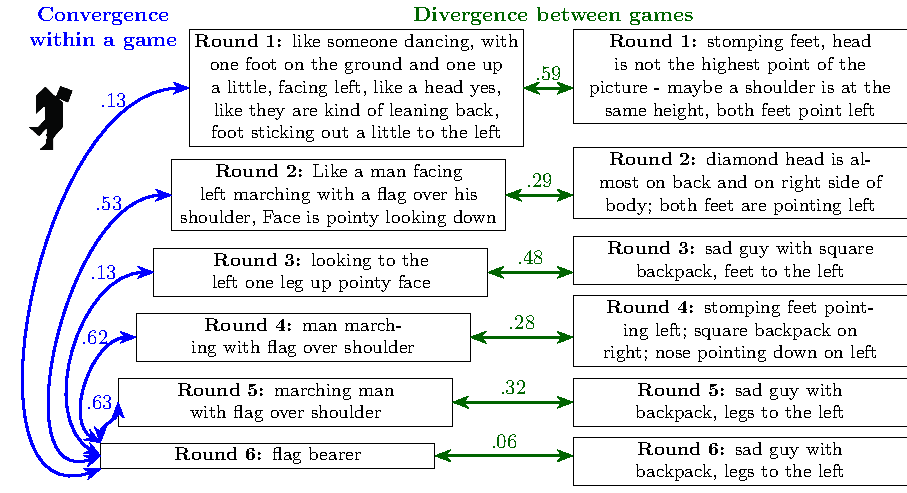
\includegraphics[width=1\linewidth]{sbert} 

}

\caption{Example utterances describing the shown tangram figure produced by two 3-player games in Experiment 1. To measure convergence within a game (blue), we measured the cosine similarity between SBERT embeddings of descriptions and the embedding of the round 6 utterance (taken to be the convention). Higher cosine similarity indicates more similar meaning. To measure divergence between games (green), we measured the similarity between utterances from the same round across games.}\label{fig:sbert-diagram}
\end{figure*}

In addition to behavioral measures, we looked at how the speaker's descriptions changed over time within and between games. We concatenated speaker's messages within a trial and used SBERT to embed the description into a high-dimensional vector space {[}TODO CITE{]}. We can compare the similarity between a pair of utterances by using the cosine similarity between their embeddings.

As a measure of convention formation, we tracked how utterances describing the same tangram in the same game become increasingly similar over the course of a game. If conventions are forming we expect the similarity to the last block utterance to increase over the course of the game. If different games go in different directions with their descriptions, we'd expect this similarity between descriptions of the same image in different games to decrease over repetitions. These two metrics are illustrated with examples in Figure \ref{fig:sbert-diagram}.

\begin{figure*}[t!]

{\centering \includegraphics[width=1\linewidth]{figs/sbert-1} 

}

\caption{Language similarity results measured with pairwise cosine similarity between embeddings of two utterances. A. Convergence of utterances within games as measured by similarity between an utterance from block 1-5 to the block 6 utterance in the same game for the same image. Dots are per-game averages, smooths are quadratic. B. Divergence of utterances across games as measured by the similarity between an utterances and utterances produced for the same image by different groups in the same block. Dots are per-image averages, smooths are quadratic.}\label{fig:sbert}
\end{figure*}

To measure convergence, we compared utterances from the first 5 blocks of a game to the ``convention'' or last block utterance for the same figure. As visible in Figure \ref{fig:sbert}A, increasing similarity the last block utterance occurs across all conditions. In experiment 1, the starting similarity of the first utterance to the last last utterance is invariant across group size (-0.008 {[}-0.021, 0.005{]}), but for smaller groups, similarity increases rapidly and they converge faster (-0.008 {[}-0.011, -0.005{]}). Convergence was especially rapid in the experiment 2 single speaker condition (0.086 {[}0.078, 0.094{]}) where all the utterances come from the same person. In experiment 3, convergence is slower in thin games than thick games (-0.025 {[}-0.033, -0.017{]}) and especially thin 6 player games (-0.035 {[}-0.047, -0.025{]}). This convergence towards the last utterance is made up of a cumulative increasing similarity between pairs of adjacent utterances (i.e.~blocks 5 and 6 are closer to each other than block 1 is to 2). TODO SEE SUPPLEMENT FIGURE. Not only do groups reduce the lengths of their utterances, but each group is converging towards a semantic description for the figures. This is more prominent in smaller games and games with greater group coherence.

The complement to convergence within groups is divergence between groups, as different groups develop their own ways of identifying the different figures. In experiment 1, descriptions become less similar to those used to describe the same figure in other games (-0.035 {[}-0.038, -0.032{]}). Group size does not affect the cross-groups similarities in the first block (0.002 {[}0, 0.004{]}), but smaller groups diverge from each other faster than larger groups (0.001 {[}0.001, 0.002{]}). In experiment 2, divergence is stronger in the single speaker (-0.041 {[}-0.043, -0.039{]}) and full feedback conditions (-0.038 {[}-0.04, -0.035{]}) than in the 6 thin condition (-0.004 {[}-0.006, -0.001{]}). In experiment 3, descriptions from different games get less similar over time in the 2-player thick condition (-0.024 {[}-0.025, -0.023{]}). The 6 player thick condition has initially higher similarity (0.051 {[}0.047, 0.055{]}, but diverges faster (-0.008 {[}-0.01, -0.007{]}. The two-player thin has slightly higher similarity (0.014 {[}0.01, 0.018{]}) and slightly slower divergence (0.004 {[}0.002, 0.005{]}). Most noticeably, the 6 player thin games diverge much more slowly than the other conditions (0.017 {[}0.015, 0.019{]}).

As group narrow in on descriptions for each image that differ from other groups, the names for each tangram differentiate with a group (See supp figure TODO).

These semantic patterns are all consistent with the partner-specific convention development and differentiation proposed by CITE someone must have verbally described the pattern.

\hypertarget{general-discussion}{%
\section{General Discussion}\label{general-discussion}}

We often communicate with multiple people at once, but much of the research on communication has been on dyads. One common paradigm for studying communication has been iterated reference games, where the phenomenon of reduction over repeated reference has been robustly established.

We build on this tradition by expanding the reference game paradigm to larger groups under various interaction structures. Across 3 online experiments and 11 experimental conditions, we varied game features including group size, form of listener backchannel, and degree of group coherence. All conditions shows the same patterns of increasing accuracy, reduction in speaker utterances, and semantic convergence within and divergence between groups. Thus, the classic reduction phenomena can occur even under situations with constrained interaction structure.

However, the interaction stucture of a group affects how rapidly groups converge to partner-specific conventions, whether measured via reduction or via semantic convergence. Smaller groups and games with thicker communication channels converged faster and more robustly than games that were larger or had thinner communication channels. These factors add together to form the overall group experience. We can interpret the experiment 3 pattern as saying that 2-player games can cope with limited feedback mechanisms, but 6-player games suffer without access to more feedback.

The 6 thin condition also presents intriguing evidence that reduction and partner-specific utterance formation might not be closely tethered: this condition shows reduction that is not substantially different than in the 6 thick condition, but it shows much less semantic convergence than other conditions. This is just one condition, but it suggests that descriptions can shorten without differentiating, perhaps all shortening to a common prior. CITE THAT PAPER ABOUT GROUP SIZE This highlights the importance of measuring semantics separately from just length proxies.
Our goal here was to further explore the space; not to directly adjudicate theories. However, given how little listeners talked, and the success of games where listeners had a limited backchannel, it seems that people are readily able to jointly agree on conventions without talking (consistent with RSA-etc CITATIONS models).

Overall, we have a number of groups, and a large corpus of language that could be probed further. The number of groups in any one condition is limited, but overall, there's a lot of people and a lot of language. TODO needs work

{[}not sure if/where to include{]} My biggest take away from this is that the hard part seems to be getting first contact with a shared meaning (and knowing you have done this), and the ``reducing'' part is easier since you have something to work with. So, how ideas of how to describe are sampled might be worth exploring more?

\hypertarget{limitations}{%
\subsection{Limitations}\label{limitations}}

Communication is a highly complex beast, so this set of experiments only explored a small part of the domain. Even just the general framework of iterated reference, there is a high dimensional feature space of possible experiments. We sampled only a few points along a few dimensions in the space. In our experiment 3, we grouped some factors together in order to have more groups in each condition: a fully factorial design would have been too expensive to power adequately. One dimension we did not vary was targets, where we stuck with the same tangram figures used in prior experiments. Thus, some of the patterns of reduction may be particular to the level of unnameable yet evocative and describable that these figures are, and not present with more or less conventional stimuli.

Group to group variability is high, as individual differences in communication style and shape description ability interacted. Coupled with small numbers of groups in some conditions, measures may be somewhat noisy depending on the random assignment of participants to games and conditions.

We cannot make claims about causal mechanisms between how experimental set-ups such as group size resulted in different outcomes: for instance, there are many differences between being in a 2-person group versus a 6-person group that could lead to the different outcomes. In a dyad, speakers can tailor their utterances to the one listener, but in large groups, speakers must balance the competing needs of different listeners (\protect\hyperlink{ref-schober1989}{Schober \& Clark 1989}, \protect\hyperlink{ref-tolins2016}{Tolins \& Fox Tree 2016}). These effects likely vary by both the knowledge state of and communication channels available to the listeners (\protect\hyperlink{ref-horton2002}{Horton \& Gerrig 2002}, \protect\hyperlink{ref-horton2005}{Horton \& Gerrig 2005}, \protect\hyperlink{ref-fox-tree2013}{Fox Tree \& Clark 2013}).

How does this controlled experimental condition map onto the real world? Group dynamics vary widely, and different dynamics scale differently with group size. In the experiment, listeners could not see each others answers while they were selecting, while in some real world situations, listeners might be able to collaborate and see what others are reaching towards. In these settings with more shared common ground and the ability to quickly learn from others success, group size might be more advantageous than in this setting.

Group interactions are rich, and this experiment is necessarily a schematic simplification with a number of limitations. Real-life situations vary widely in who the interlocuters are, their relationships, their goals, and their environment (\protect\hyperlink{ref-carletta1998}{Carletta et al. 1998}, \protect\hyperlink{ref-fay2000}{Fay et al. 2000}). Our participants were a convenience sample of Prolific workers who were strangers to each other; thus we miss richness that could come from prior relationships or shared community. Reference is only one goal out of many possible communicative goals, and the tangram images are artificial.

\hypertarget{conclusion}{%
\subsection{Conclusion ??}\label{conclusion}}

TODO

\hypertarget{methods}{%
\section{Methods}\label{methods}}

For all experiments, we used Empirica (\protect\hyperlink{ref-almaatouqEmpiricaVirtualLab2020}{Almaatouq et al. 2020}) to create real-time multi-player reference games. In each game, one of the players started as the speaker who saw an array of tangrams with one highlighted (Figure \ref{game}A) and communicated which figure to click to the other players (listeners). After the speaker had identified each of the 12 images in turn, the process repeated with the same images, but a total of 6 blocks (72 trials). We recorded what participants said in the chat, as well as who selected what image and how long they took to make their selections.

These experiments were designed sequentially and pre-registered individually.\footnote{Experiment 1: \url{https://osf.io/cn9f4} for the 2-4 player groups, and \url{https://osf.io/rpz67} for the 5-6 player data run later. Experiment 2: single speaker at \url{https://osf.io/f9xyd}, full feedback at \url{https://osf.io/j5zbm}, and thin at \url{https://osf.io/k5f4t}. Experiment 3: \url{https://osf.io/untzy}} We followed the analysis plan, although additional analyses were added to early experiments that were only pre-registered in later experiments. Some pre-registered models were omitted from the main text, but are shown in the supplement TODO.

\hypertarget{participants}{%
\subsection{Participants}\label{participants}}

\begin{table}

\caption{\label{tab:participants}The number of games in each experiment and condition. Complete games finished all 6 blocks; partial games ended early due to disconnections, but contributed at least one complete block of data. 6* indicates that some games started with fewer than 6 players or continued with fewer than 6 players after participants disconnected.}
\centering
\begin{tabular}[t]{l|l|r|r|r}
\hline
Experiment & Players & Complete & Partial & Total Participants\\
\hline
1: baseline & 2 & 15 & 4 & 38\\
\hline
1: baseline & 3 & 18 & 2 & 60\\
\hline
1: baseline & 4 & 19 & 2 & 84\\
\hline
1: baseline & 5 & 17 & 3 & 100\\
\hline
1: baseline & 6 & 12 & 6 & 108\\
\hline
2: single speaker & 6 & 15 & 3 & 108\\
\hline
2: full feedback & 6 & 13 & 4 & 102\\
\hline
2: thin & 6 & 10 & 6 & 96\\
\hline
3: thin & 2 & 35 & 3 & 76\\
\hline
3: thin & 6* & 44 & 0 & 235\\
\hline
3: thick & 2 & 39 & 3 & 84\\
\hline
3: thick & 6* & 38 & 2 & 222\\
\hline
\end{tabular}
\end{table}

Participants were recruited using the Prolific platform, and all participants self-reported as fluent native English speakers on Prolific's demographic prescreen. Participants each took part in only one experiment. Experiment 1 took place between May and July 2021, experiment 2 between March and August 2022, and experiment 3 in October 2022. As games varied in length depending on the number of participants, we paid participants based on group size, with the goal of a \$10 hourly rate. Participants were paid \$7 for 2-player games, \$8.50 for 3-player games, \$10 for 4-player games, and \$11 for 5- and 6-player games. When one player had the speaker role for the entirety of a 6-player game, they gained an addition \$2 bonus. Across all games, each participant could early up to \$2.88 in performance bonuses. A total of 1319 people participated across the 3 experiments. A breakdown of number of games and participants in each condition is shown in Table \ref{tab:participants}.

\hypertarget{materials}{%
\subsection{Materials}\label{materials}}

We used the 12 tangram images used by Hawkins et al. (\protect\hyperlink{ref-hawkinsCharacterizingDynamicsLearning2020}{2020}) and Clark \& Wilkes-Gibbs (\protect\hyperlink{ref-clarkReferringCollaborativeProcess1986}{1986}) (see Figure \ref{game}). These images were displayed in a grid with order randomized for each participant (thus descriptions such as ``top left'' were ineffective as the image might be in a different place on the speaker's and listeners' screens). The same images were used every block.

\hypertarget{procedure}{%
\subsection{Procedure}\label{procedure}}

The experimental procedure was very similar across the three experiments. We first describe the procedure used in experiment 1 and then describe the differences in later experiments.

\hypertarget{experiment-1}{%
\subsubsection{Experiment 1}\label{experiment-1}}

We implemented the experiment using Empirica, a Javascript-based platform for running real-time interactive experiments online (\protect\hyperlink{ref-almaatouqEmpiricaVirtualLab2020}{Almaatouq et al. 2020}). From Prolific, participants were directed to our website where they navigated through a self-paced series of instruction pages explaining the game. Participants had to pass a quiz to be able to play the game. They were then directed to a ``waiting room'' screen until their partners were ready.

Once the game started, participants saw screens like Figure \ref{game}A. Each trial, the speaker described the highlighted tangram image so that the listeners could identify and click it. All participants were free to use the chat box to communicate, but listeners could only click once the speaker had sent a message. Once a listener clicked, they could not change their selection. There was no signal to the speaker or other listeners about who had already made a selection.

Once all listeners had selected (or a 3-minute timer ran out), participants were given feedback (Figure \ref{game}B). Listeners learned whether they individually had chosen correctly or not; listeners who were incorrect were not told the correct answer. The speaker saw which tangram each listener had selected, but listeners did not. Listeners got 4 points for each correct answer; the speaker got points equal to the average of the listeners' points. These points translated into performance bonus at the end of the experiment.

In each block, each of the 12 tangrams was indicated to the speaker once. The same person was the speaker for an entire block, but participants rotated roles between blocks. Thus, over the course of the 6 blocks, participants were speakers 3 times in 2-player games, twice in 3-player games, once or twice in 4 and 5-player games, and once in 6-player games. Rotating the speaker was chosen to keep participants more equally engaged (the speaker role is more work), and to give a more robust test for reduction and convention.

After the game finished, participants were given a survey asking for optional demographic information and feedback on their experience with the game.

\hypertarget{differences-in-experiment-2}{%
\subsubsection{Differences in experiment 2}\label{differences-in-experiment-2}}

Experiment 2 consisted of three different variations on Experiment 1, all conducted in 6 player games. Each of these conditions differed from the experiment 1 baseline in one way. The single speaker condition differed only in that one person was designated the speaker for the entire game, rather than having the speaker role rotate. The full feedback condition differed from experiment 1 in that all participants were shown what each person had selected and what the right answer was; listeners still saw text saying whether they individually were right or wrong. This was similar to some dyadic work, such as Hawkins et al. (\protect\hyperlink{ref-hawkinsCharacterizingDynamicsLearning2020}{2020}) where listeners were shown what the right answer was during feedback. For the thin condition, we altered the chatbox interface for listeners. Instead of a textbox, listeners had 4 buttons, each of which sent a different emoji to the chat. Listeners were given suggested meanings for the 4 emojis during instructions. They could send the emojis as often as desired, for instance, initially indicating confusion, and later indicating understanding. In addition, we added notifications that appeared in the chat box saying when a player had made a selection.

\hypertarget{differences-in-experiment-3}{%
\subsubsection{Differences in experiment 3}\label{differences-in-experiment-3}}

The thin channel condition in experiment 3 was the same as the thin condition in experiment 2, above. The thick condition combined the two group coherency enhancing variations from experiment 2: one person was the designated speaker throughout, and the feedback participants received included the right answer and what each player had selected. Across both conditions in experiment 3, notifications were sent to the chat to indicate when a participant had made a selection.

\hypertarget{data-pre-processing-and-exclusions}{%
\subsection{Data pre-processing and exclusions}\label{data-pre-processing-and-exclusions}}

Participants could use the chat box freely, which meant that the chat transcript contained some non-referential language. The first author skimmed through the chat transcripts, tagging utterances that did not refer to the current tangram. These were primarily pleasantries (``Hello''), meta-commentary about how well or fast the task was going, and confirmations or denials (``ok'', ``got it'', ``yes'', ``no''). We exclude these utterances from our analyses. Note that chat lines sometimes included non-referential words in addition to words referring to the tangrams (``ok, so it looks like a zombie'', ``yes, the one with legs''); these lines were retained intact.

In experiments 1 and 2, games did not start if there were not enough participants and ended if any participant disconnected. In experiment 3, games started after a waiting period even if they were not full and continued even after a participant disconnected (with speaker role reassigned if necessary), unless the game would drop below 2 players. The distribution of playes in these 6* player games is at TODO SUPPLEMENT! The realities of online recruitment and disconnection meant that the number of games varied, although we aimed for 20 games in each condition in experiments 1 and 2, and 40 per condition in experiment 3. We excluded incomplete blocks from analyses, but included complete blocks from partial games (See Table \ref{tab:participants} for counts).

When skimming transcripts to tag non-referential utterances, we noticed that one game in the 6-player thick game had a speaker who did not give any sort of coherent descriptions, even with substantial listener prompting. We excluded this game from analyses.

\hypertarget{modelling-strategy}{%
\subsection{Modelling strategy}\label{modelling-strategy}}

In experiment 3, some of the 6 player games did not have 6 players for the entire game. We do not model this, as it is unclear at what point in the game group size is most relevant. We note that this is a conservative choice that will underestimate differences between 2 player and (genuine) 6 player games, by labelling some smaller groups as 6 player.

We ran all models in brms (CITE) with weakly regularizing priors. We were often unable to fit the full mixed effects structure that we had pre-registered in a reasonable amount of time, so we included what heirarchical effects were reasonable. (All model results and priors and formulae are reported in TODO supplement). Accuracy results used a logistic model, other results use linear models. Accuracy models were all run as logistic models with normal(0,1) priors for both betas and sd. Reduction models were run as linear models with an intercept prior of normal(12,20), a beta prior of normal(0,10), an sd prior of normal(0,5) and a correlation prior of lkj(1). For all of the models of sbert similarity, we used linear models with the priors normal(.5,.2) for intercept, normal(0,.1) for beta, and normal(0,.05) for sd.

\hypertarget{supplement}{%
\section{Supplement}\label{supplement}}

This supplement will get moved to a separate file, but for now is tacked on.

\hypertarget{figures-of-listener-performance}{%
\subsection{Figures of listener performance}\label{figures-of-listener-performance}}

\begin{figure*}[t!]

{\centering \includegraphics[width=1\linewidth]{figs/emoji-1} 

}

\caption{Fraction of trials on which at least one listener produced the labelled emoji (or any emoji.}\label{fig:emoji}
\end{figure*}

\begin{figure*}[t!]

{\centering \includegraphics[width=1\linewidth]{figs/listeners-1} 

}

\caption{Number of words of referential language produced by listeners over time. Excludes trials where no listeners contributed descriptive language.  }\label{fig:listeners}
\end{figure*}

\begin{figure*}[t!]

{\centering \includegraphics[width=1\linewidth]{figs/listeners2-1} 

}

\caption{Fraction of trials when any reference language (or emoji) was produced by any listener.}\label{fig:listeners2}
\end{figure*}

\begin{figure*}[t!]

{\centering \includegraphics[width=1\linewidth]{figs/other-1} 

}

\caption{Additional measures of convergence and divergence. A is similarity to first utterance. B is similarity between utterances from adjacent blocks. C is divergence in descriptions of different tangrams within a group}\label{fig:other}
\end{figure*}

\hypertarget{distinctiveness-of-tangrams}{%
\subsection{Distinctiveness of tangrams}\label{distinctiveness-of-tangrams}}

Another way of looking at how language changes over the course of the game is looking at how games start to refer to different tangrams more differently. This could reflect initial overlap in descriping many figures as sitting or standing or by leg and arm and head position.

Over the course of the game, descriptions for each tangram become more distinctive (-0.043 {[}-0.046, -0.039{]}).
In all three subexperiments, the descriptions of tangrams become more distinctive within games across time. (2a -0.046 {[}-0.048, -0.044{]}, 2b -0.025 {[}-0.028, -0.022{]}, 2c -0.025 {[}-0.028, -0.022{]}).

Tangram distinctiveness within games increased over time (-0.027 {[}-0.029, -0.025{]}). There might be more to say about other effects, but it's mostly a starting places being different in larger games and then the slopes also differ a bit?

\hypertarget{play-with-more-diagrams}{%
\subsubsection{play with more diagrams}\label{play-with-more-diagrams}}

Comparing utterances between adjacent rounds reveals similar patterns. Thin games have lower similarity between adjacent blocks (-0.124 {[}-0.159, -0.088{]}) as do larger games (-0.034 {[}-0.069, 0.003{]}). Later in the game adjacent blocks are more similar than earlier adjacent blocks (0.046 {[}0.041, 0.052{]}), painting an overall nonlinear convergent pattern (as seen in Figure \ref{fig:other}).

\hypertarget{accuracy-models}{%
\subsection{Accuracy models}\label{accuracy-models}}

Accuracy models were all run as logistic models with normal(0,1) priors for both betas and sd. This model was not explicitly included in the experiment 1 and 2 pre-registrations; it was included with more ambitious mixed effects (which did not run in a timely manner) in the experiment 3 pre-reg.

\begin{table}[h!]

\caption{\label{tab:unnamed-chunk-11}Experiment 1 logistic model of listener accuracy:\\ correct.num~$\sim$ block~$\times$ numPlayers~+ (1|gameId)}
\centering
\begin{tabular}[t]{lll}
\toprule
Term & Est. & CrI\\
\midrule
block & 0.44 & {}[0.31, 0.58]\\
block:numPlayers & -0.02 & {}[-0.05, 0.01]\\
Intercept & 2.10 & {}[1.57, 2.65]\\
numPlayers & -0.07 & {}[-0.2, 0.05]\\
\bottomrule
\end{tabular}
\end{table}

\begin{table}[h!]

\caption{\label{tab:unnamed-chunk-11}Experiment 2: 6 single speaker logistic model of listener accuracy:\\ correct.num~$\sim$ block~+ (1|gameId)}
\centering
\begin{tabular}[t]{lll}
\toprule
Term & Est. & CrI\\
\midrule
block & 0.45 & {}[0.39, 0.52]\\
Intercept & 1.78 & {}[1.4, 2.19]\\
\bottomrule
\end{tabular}
\end{table}

\begin{table}[h!]

\caption{\label{tab:unnamed-chunk-11}Experiment 2: 6 full feedback logistic model of listener accuracy:\\ correct.num~$\sim$ block~+ (1|gameId)}
\centering
\begin{tabular}[t]{lll}
\toprule
Term & Est. & CrI\\
\midrule
block & 0.47 & {}[0.39, 0.54]\\
Intercept & 1.35 & {}[0.59, 2.06]\\
\bottomrule
\end{tabular}
\end{table}

\begin{table}[h!]

\caption{\label{tab:unnamed-chunk-11}Experiment 2: 6 thin logistic model of listener accuracy:\\ correct.num~$\sim$ block~+ (1|gameId)}
\centering
\begin{tabular}[t]{lll}
\toprule
Term & Est. & CrI\\
\midrule
block & 0.23 & {}[0.19, 0.28]\\
Intercept & 0.88 & {}[0.64, 1.12]\\
\bottomrule
\end{tabular}
\end{table}

\begin{table}[h!]

\caption{\label{tab:unnamed-chunk-11}Experiment 3 logistic model of listener accuracy:\\ correct.num~$\sim$ block~$\times$ gameSize~$\times$ channel~+ (1|gameId)}
\centering
\begin{tabular}[t]{lll}
\toprule
Term & Est. & CrI\\
\midrule
block & 0.41 & {}[0.32, 0.5]\\
block:channelthin & -0.07 & {}[-0.18, 0.04]\\
block:gameSize6 & -0.34 & {}[-0.43, -0.25]\\
block:gameSize6:channelthin & 0.07 & {}[-0.05, 0.19]\\
channelthin & -0.36 & {}[-0.78, 0.05]\\
\addlinespace
gameSize6 & -0.64 & {}[-1.05, -0.25]\\
gameSize6:channelthin & 0.31 & {}[-0.22, 0.87]\\
Intercept & 1.69 & {}[1.39, 1.99]\\
\bottomrule
\end{tabular}
\end{table}

\pagebreak

\hypertarget{reduction-models}{%
\subsection{Reduction models}\label{reduction-models}}

Reduction models were run as linear models with an intercept prior of normal(12,20), a beta prior of normal(0,10), an sd prior of normal(0,5) and a correlation prior of lkj(1). This model was pre-registered for each experiment and run with the mixed effects structure as prespecified.

\begin{table}[h!]

\caption{\label{tab:unnamed-chunk-12}Experiment 1:\\ words~$\sim$ block~$\times$ numPlayers~+ (block|tangram)~+ (1|playerId)~+ (1|tangram:gameId)~+ (block|gameId)}
\centering
\begin{tabular}[t]{lll}
\toprule
Term & Est. & CrI\\
\midrule
block & -3.37 & {}[-4.54, -2.24]\\
block:numPlayers & -0.10 & {}[-0.36, 0.17]\\
Intercept & 16.79 & {}[11.96, 21.93]\\
numPlayers & 1.66 & {}[0.66, 2.61]\\
\bottomrule
\end{tabular}
\end{table}

\begin{table}[h!]

\caption{\label{tab:unnamed-chunk-12}Experiment 2: 6 single speaker:\\ words~$\sim$ block~+ (block|tangram)~+ (1|tangram:gameId)~+ (block|gameId)}
\centering
\begin{tabular}[t]{lll}
\toprule
Term & Est. & CrI\\
\midrule
block & -5.39 & {}[-6.46, -4.31]\\
Intercept & 29.93 & {}[24.92, 34.84]\\
\bottomrule
\end{tabular}
\end{table}

\begin{table}[h!]

\caption{\label{tab:unnamed-chunk-12}Experiment 2: 6 full feedback:\\ words~$\sim$ block~+ (block|tangram)~+ (1|tangram:gameId)~+ (block|gameId)}
\centering
\begin{tabular}[t]{lll}
\toprule
Term & Est. & CrI\\
\midrule
block & -4.68 & {}[-5.88, -3.52]\\
Intercept & 26.03 & {}[21.12, 30.58]\\
\bottomrule
\end{tabular}
\end{table}

\begin{table}[h!]

\caption{\label{tab:unnamed-chunk-12}Experiment 2: 6 thin:\\ words~$\sim$ block~+ (block|tangram)~+ (1|tangram:gameId)~+ (block|gameId)}
\centering
\begin{tabular}[t]{lll}
\toprule
Term & Est. & CrI\\
\midrule
block & -2.15 & {}[-3.44, -1.12]\\
Intercept & 20.50 & {}[17.26, 23.76]\\
\bottomrule
\end{tabular}
\end{table}

\begin{table}[h!]

\caption{\label{tab:unnamed-chunk-12}Experiment 3:\\ words~$\sim$ block~$\times$ channel~$\times$ gameSize~+ (block~$\times$ channel~$\times$ gameSize|tangram)~+ (1|tangram:gameId)~+ (block|gameId)}
\centering
\begin{tabular}[t]{lll}
\toprule
Term & Est. & CrI\\
\midrule
block & -2.29 & {}[-2.95, -1.6]\\
block:channelthin & 0.32 & {}[-0.65, 1.24]\\
block:channelthin:gameSize6 & 0.64 & {}[-0.61, 1.89]\\
block:gameSize6 & -1.21 & {}[-2.06, -0.3]\\
channelthin & 0.63 & {}[-3.18, 4.73]\\
\addlinespace
channelthin:gameSize6 & -2.11 & {}[-7.41, 2.98]\\
gameSize6 & 7.41 & {}[3.57, 11.18]\\
Intercept & 14.99 & {}[11.86, 17.89]\\
\bottomrule
\end{tabular}
\end{table}

\hypertarget{extra-reduction-model}{%
\subsubsection{Extra reduction model}\label{extra-reduction-model}}

For experiment 1, we also pre-specified models about whether the speaker's correctness (as a listener) on the prior block had an effect

Model of whether speaker's correct/incorrect answer in previous block has an effect -

words \textasciitilde{} block\emph{player\_count + block}was\_correct+ (block\textbar tangram) + (1\textbar speaker)
+ (1\textbar tangram*group)+(block\textbar group)

TODO

\begin{verbatim}
## [1] "words~$\\sim$ block~$\\times$ numPlayers~+ block~$\\times$ wasINcorrect~+ (block|tangram)~+ (1|playerId)~+ (1|tangram:gameId)~+ (block|gameId)"
\end{verbatim}

\begin{table}[h!]

\caption{\label{tab:unnamed-chunk-13}Experiment 1:\\ words~$\sim$ block~$\times$ numPlayers~+ block~$\times$ wasINcorrect~+ (block|tangram)~+ (1|playerId)~+ (1|tangram:gameId)~+ (block|gameId)}
\centering
\begin{tabular}[t]{lll}
\toprule
Term & Est. & CrI\\
\midrule
block & -2.15 & {}[-3.35, -0.98]\\
block:numPlayers & -0.23 & {}[-0.51, 0.06]\\
block:wasINcorrect & 0.25 & {}[-0.24, 0.74]\\
Intercept & 11.98 & {}[6.31, 17.7]\\
numPlayers & 2.15 & {}[0.93, 3.36]\\
\addlinespace
wasINcorrect & 3.08 & {}[1.69, 4.42]\\
\bottomrule
\end{tabular}
\end{table}

\hypertarget{listener-models}{%
\subsubsection{Listener models}\label{listener-models}}

\begin{table}[h!]

\caption{\label{tab:unnamed-chunk-14}Experiment 1:\\ words~$\sim$ block~$\times$ numPlayers~+ (block|gameId)}
\centering
\begin{tabular}[t]{lll}
\toprule
Term & Est. & CrI\\
\midrule
block & -0.17 & {}[-1.63, 1.24]\\
block:numPlayers & -0.41 & {}[-0.72, -0.09]\\
Intercept & 4.67 & {}[0.09, 9.32]\\
numPlayers & 2.12 & {}[1.03, 3.12]\\
\bottomrule
\end{tabular}
\end{table}

\begin{table}[h!]

\caption{\label{tab:unnamed-chunk-14}Experiment 1:\\ is.words~$\sim$ block~$\times$ numPlayers~+ (1|gameId)}
\centering
\begin{tabular}[t]{lll}
\toprule
Term & Est. & CrI\\
\midrule
block & -0.80 & {}[-0.97, -0.63]\\
block:numPlayers & 0.03 & {}[0, 0.07]\\
Intercept & -2.65 & {}[-3.5, -1.83]\\
numPlayers & 0.78 & {}[0.58, 0.98]\\
\bottomrule
\end{tabular}
\end{table}
\pagebreak

\hypertarget{sbert-models}{%
\subsection{SBERT models}\label{sbert-models}}

For all of the models of sbert similarity, we used linear models with the priors normal(.5,.2) for intercept, normal(0,.1) for beta, and normal(0,.05) for sd.

These models were verbally described (but not formally specified) in the pre-registrations for experiment 2 in the full feedback and thin conditions and for experiment 3, for looking at divergence between games, convergence within games (compare to first, next, and last), and divergence between tangrams within games.

\hypertarget{convergence-within-games-comparison-to-last-round}{%
\subsubsection{Convergence within games: comparison to last round}\label{convergence-within-games-comparison-to-last-round}}

This is the convergence metric presented in the paper.

\begin{table}[h!]

\caption{\label{tab:unnamed-chunk-15}Experiment 1:\\ sim~$\sim$ earlier~$\times$ condition~+ (1|tangram)~+ (1|gameId)}
\centering
\begin{tabular}[t]{lll}
\toprule
Term & Est. & CrI\\
\midrule
condition & -0.01 & {}[-0.02, 0]\\
earlier & 0.09 & {}[0.08, 0.1]\\
earlier:condition & -0.01 & {}[-0.01, -0.01]\\
Intercept & 0.52 & {}[0.46, 0.57]\\
\bottomrule
\end{tabular}
\end{table}

\begin{table}[h!]

\caption{\label{tab:unnamed-chunk-15}Experiment 2: 6 single speaker:\\ sim~$\sim$ earlier~+ (1|tangram)~+ (1|gameId)}
\centering
\begin{tabular}[t]{lll}
\toprule
Term & Est. & CrI\\
\midrule
earlier & 0.09 & {}[0.08, 0.09]\\
Intercept & 0.50 & {}[0.44, 0.56]\\
\bottomrule
\end{tabular}
\end{table}

\begin{table}[h!]

\caption{\label{tab:unnamed-chunk-15}Experiment 2: 6 full feedback:\\ sim~$\sim$ earlier~+ (1|tangram)~+ (1|gameId)}
\centering
\begin{tabular}[t]{lll}
\toprule
Term & Est. & CrI\\
\midrule
earlier & 0.06 & {}[0.05, 0.07]\\
Intercept & 0.44 & {}[0.39, 0.49]\\
\bottomrule
\end{tabular}
\end{table}

\begin{table}[h!]

\caption{\label{tab:unnamed-chunk-15}Experiment 2: 6 thin:\\ sim~$\sim$ earlier~+ (1|tangram)~+ (1|gameId)}
\centering
\begin{tabular}[t]{lll}
\toprule
Term & Est. & CrI\\
\midrule
earlier & 0.02 & {}[0.01, 0.03]\\
Intercept & 0.50 & {}[0.45, 0.54]\\
\bottomrule
\end{tabular}
\end{table}

\begin{table}[h!]

\caption{\label{tab:unnamed-chunk-15}Experiment 3:\\ sim~$\sim$ earlier~$\times$ channel~$\times$ gameSize~+ (1|tangram)~+ (1|gameId)}
\centering
\begin{tabular}[t]{lll}
\toprule
Term & Est. & CrI\\
\midrule
channelthin & -0.03 & {}[-0.08, 0.01]\\
channelthin:gameSize6 & 0.04 & {}[-0.02, 0.1]\\
earlier & 0.08 & {}[0.07, 0.09]\\
earlier:channelthin & -0.02 & {}[-0.03, -0.02]\\
earlier:channelthin:gameSize6 & -0.04 & {}[-0.05, -0.02]\\
\addlinespace
earlier:gameSize6 & 0.01 & {}[0, 0.02]\\
gameSize6 & -0.07 & {}[-0.11, -0.02]\\
Intercept & 0.58 & {}[0.54, 0.62]\\
\bottomrule
\end{tabular}
\end{table}

\pagebreak

\hypertarget{divergence-across-games}{%
\subsubsection{Divergence across games}\label{divergence-across-games}}

To look at how games diverged from each other \ldots{} TODO

\begin{table}[h!]

\caption{\label{tab:unnamed-chunk-16}Experiment 1:\\ sim~$\sim$ block~$\times$ condition~+ (1|tangram)}
\centering
\begin{tabular}[t]{lll}
\toprule
Term & Est. & CrI\\
\midrule
block & -0.04 & {}[-0.04, -0.03]\\
block:condition & 0.00 & {}[0, 0]\\
condition & 0.00 & {}[0, 0]\\
Intercept & 0.47 & {}[0.43, 0.51]\\
\bottomrule
\end{tabular}
\end{table}

\begin{table}[h!]

\caption{\label{tab:unnamed-chunk-16}Experiment 2: 6 single speaker:\\ sim~$\sim$ block~+ (1|tangram)}
\centering
\begin{tabular}[t]{lll}
\toprule
Term & Est. & CrI\\
\midrule
block & -0.04 & {}[-0.04, -0.04]\\
Intercept & 0.48 & {}[0.44, 0.53]\\
\bottomrule
\end{tabular}
\end{table}

\begin{table}[h!]

\caption{\label{tab:unnamed-chunk-16}Experiment 2: 6 full feedback:\\ sim~$\sim$ block~+ (1|tangram)}
\centering
\begin{tabular}[t]{lll}
\toprule
Term & Est. & CrI\\
\midrule
block & -0.04 & {}[-0.04, -0.04]\\
Intercept & 0.50 & {}[0.46, 0.55]\\
\bottomrule
\end{tabular}
\end{table}

\begin{table}[h!]

\caption{\label{tab:unnamed-chunk-16}Experiment 2: 6 thin:\\ sim~$\sim$ block~+ (1|tangram)}
\centering
\begin{tabular}[t]{lll}
\toprule
Term & Est. & CrI\\
\midrule
block & 0.00 & {}[-0.01, 0]\\
Intercept & 0.43 & {}[0.41, 0.46]\\
\bottomrule
\end{tabular}
\end{table}

\begin{table}[h!]

\caption{\label{tab:unnamed-chunk-16}Experiment 3:\\ sim~$\sim$ block~$\times$ channel~$\times$ gameSize~+ (1|tangram)}
\centering
\begin{tabular}[t]{lll}
\toprule
Term & Est. & CrI\\
\midrule
block & -0.02 & {}[-0.02, -0.02]\\
block:channelthin & 0.00 & {}[0, 0]\\
block:channelthin:gameSize6 & 0.02 & {}[0.02, 0.02]\\
block:gameSize6 & -0.01 & {}[-0.01, -0.01]\\
channelthin & 0.01 & {}[0.01, 0.02]\\
\addlinespace
channelthin:gameSize6 & -0.03 & {}[-0.04, -0.02]\\
gameSize6 & 0.05 & {}[0.05, 0.05]\\
Intercept & 0.41 & {}[0.37, 0.45]\\
\bottomrule
\end{tabular}
\end{table}

\pagebreak

\hypertarget{divergence-across-tangrams}{%
\subsubsection{Divergence across tangrams}\label{divergence-across-tangrams}}

\begin{table}[h!]

\caption{\label{tab:unnamed-chunk-17}Experiment 1:\\ sim~$\sim$ block~$\times$ condition~+ (1|gameId)}
\centering
\begin{tabular}[t]{lll}
\toprule
Term & Est. & CrI\\
\midrule
block & -0.04 & {}[-0.05, -0.04]\\
block:condition & 0.00 & {}[0, 0]\\
condition & 0.00 & {}[-0.01, 0.01]\\
Intercept & 0.43 & {}[0.38, 0.47]\\
\bottomrule
\end{tabular}
\end{table}

\begin{table}[h!]

\caption{\label{tab:unnamed-chunk-17}Experiment 2: 6 single speaker:\\ sim~$\sim$ block~+ (1|gameId)}
\centering
\begin{tabular}[t]{lll}
\toprule
Term & Est. & CrI\\
\midrule
block & -0.05 & {}[-0.05, -0.04]\\
Intercept & 0.42 & {}[0.39, 0.44]\\
\bottomrule
\end{tabular}
\end{table}

\begin{table}[h!]

\caption{\label{tab:unnamed-chunk-17}Experiment 2: 6 full feedback:\\ sim~$\sim$ block~+ (1|gameId)}
\centering
\begin{tabular}[t]{lll}
\toprule
Term & Est. & CrI\\
\midrule
block & -0.05 & {}[-0.05, -0.04]\\
Intercept & 0.46 & {}[0.42, 0.5]\\
\bottomrule
\end{tabular}
\end{table}

\begin{table}[h!]

\caption{\label{tab:unnamed-chunk-17}Experiment 2: 6 thin:\\ sim~$\sim$ block~+ (1|gameId)}
\centering
\begin{tabular}[t]{lll}
\toprule
Term & Est. & CrI\\
\midrule
block & -0.03 & {}[-0.03, -0.02]\\
Intercept & 0.43 & {}[0.39, 0.47]\\
\bottomrule
\end{tabular}
\end{table}

\begin{table}[h!]

\caption{\label{tab:unnamed-chunk-17}Experiment 3:\\ sim~$\sim$ block~$\times$ channel~$\times$ gameSize~+ (1|gameId)}
\centering
\begin{tabular}[t]{lll}
\toprule
Term & Est. & CrI\\
\midrule
block & -0.03 & {}[-0.03, -0.03]\\
block:channelthin & 0.00 & {}[0, 0]\\
block:channelthin:gameSize6 & 0.01 & {}[0.01, 0.01]\\
block:gameSize6 & -0.01 & {}[-0.01, -0.01]\\
channelthin & 0.04 & {}[0, 0.08]\\
\addlinespace
channelthin:gameSize6 & -0.05 & {}[-0.11, 0]\\
gameSize6 & 0.07 & {}[0.04, 0.11]\\
Intercept & 0.38 & {}[0.35, 0.4]\\
\bottomrule
\end{tabular}
\end{table}

\pagebreak

\hypertarget{convergence-to-next}{%
\subsubsection{convergence to next}\label{convergence-to-next}}

We also looked at how similar an utterance was to the next round utterance: this can be thought of as the derivative of the to-last comparison. (although cosine similarities are not actually additive in the same way integrals are)

\begin{table}[h!]

\caption{\label{tab:unnamed-chunk-18}Experiment 1:\\ sim~$\sim$ earlier~$\times$ condition~+ (1|tangram)~+ (1|gameId)}
\centering
\begin{tabular}[t]{lll}
\toprule
Term & Est. & CrI\\
\midrule
condition & 0.00 & {}[-0.01, 0.01]\\
earlier & 0.06 & {}[0.05, 0.07]\\
earlier:condition & -0.01 & {}[-0.01, -0.01]\\
Intercept & 0.59 & {}[0.54, 0.64]\\
\bottomrule
\end{tabular}
\end{table}

\begin{table}[h!]

\caption{\label{tab:unnamed-chunk-18}Experiment 2: 6 single speaker:\\ sim~$\sim$ earlier~+ (1|tangram)~+ (1|gameId)}
\centering
\begin{tabular}[t]{lll}
\toprule
Term & Est. & CrI\\
\midrule
earlier & 0.04 & {}[0.04, 0.05]\\
Intercept & 0.66 & {}[0.62, 0.7]\\
\bottomrule
\end{tabular}
\end{table}

\begin{table}[h!]

\caption{\label{tab:unnamed-chunk-18}Experiment 2: 6 full feedback:\\ sim~$\sim$ earlier~+ (1|tangram)~+ (1|gameId)}
\centering
\begin{tabular}[t]{lll}
\toprule
Term & Est. & CrI\\
\midrule
earlier & 0.02 & {}[0.01, 0.02]\\
Intercept & 0.61 & {}[0.57, 0.64]\\
\bottomrule
\end{tabular}
\end{table}

\begin{table}[h!]

\caption{\label{tab:unnamed-chunk-18}Experiment 2: 6 thin:\\ sim~$\sim$ earlier~+ (1|tangram)~+ (1|gameId)}
\centering
\begin{tabular}[t]{lll}
\toprule
Term & Est. & CrI\\
\midrule
earlier & 0.01 & {}[0, 0.02]\\
Intercept & 0.53 & {}[0.49, 0.58]\\
\bottomrule
\end{tabular}
\end{table}

\begin{table}[h!]

\caption{\label{tab:unnamed-chunk-18}Experiment 3:\\ sim~$\sim$ earlier~$\times$ channel~$\times$ gameSize~+ (1|tangram)~+ (1|gameId)}
\centering
\begin{tabular}[t]{lll}
\toprule
Term & Est. & CrI\\
\midrule
channelthin & -0.12 & {}[-0.16, -0.09]\\
channelthin:gameSize6 & 0.00 & {}[-0.05, 0.05]\\
earlier & 0.05 & {}[0.04, 0.05]\\
earlier:channelthin & -0.01 & {}[-0.02, 0]\\
earlier:channelthin:gameSize6 & -0.02 & {}[-0.03, -0.01]\\
\addlinespace
earlier:gameSize6 & 0.00 & {}[-0.01, 0]\\
gameSize6 & -0.03 & {}[-0.07, 0]\\
Intercept & 0.71 & {}[0.68, 0.75]\\
\bottomrule
\end{tabular}
\end{table}

\pagebreak

\hypertarget{divergence-from-first}{%
\subsubsection{divergence from first}\label{divergence-from-first}}

We also looked at how similar an utterance was to the first round utterance. This is not very informative because first round utterances tend to be pretty unwieldy. TODO explain more or don't include

\begin{table}[h!]

\caption{\label{tab:unnamed-chunk-19}Experiment 1:\\ sim~$\sim$ later~$\times$ condition~+ (1|tangram)~+ (1|gameId)}
\centering
\begin{tabular}[t]{lll}
\toprule
Term & Est. & CrI\\
\midrule
condition & -0.01 & {}[-0.02, 0]\\
Intercept & 0.65 & {}[0.59, 0.7]\\
later & -0.03 & {}[-0.04, -0.02]\\
later:condition & 0.00 & {}[0, 0]\\
\bottomrule
\end{tabular}
\end{table}

\begin{table}[h!]

\caption{\label{tab:unnamed-chunk-19}Experiment 2: 6 single speaker:\\ sim~$\sim$ later~+ (1|tangram)~+ (1|gameId)}
\centering
\begin{tabular}[t]{lll}
\toprule
Term & Est. & CrI\\
\midrule
Intercept & 0.68 & {}[0.63, 0.73]\\
later & -0.04 & {}[-0.05, -0.03]\\
\bottomrule
\end{tabular}
\end{table}

\begin{table}[h!]

\caption{\label{tab:unnamed-chunk-19}Experiment 2: 6 full feedback:\\ sim~$\sim$ later~+ (1|tangram)~+ (1|gameId)}
\centering
\begin{tabular}[t]{lll}
\toprule
Term & Est. & CrI\\
\midrule
Intercept & 0.64 & {}[0.58, 0.71]\\
later & -0.04 & {}[-0.05, -0.04]\\
\bottomrule
\end{tabular}
\end{table}

\begin{table}[h!]

\caption{\label{tab:unnamed-chunk-19}Experiment 2: 6 thin:\\ sim~$\sim$ later~+ (1|tangram)~+ (1|gameId)}
\centering
\begin{tabular}[t]{lll}
\toprule
Term & Est. & CrI\\
\midrule
Intercept & 0.54 & {}[0.49, 0.58]\\
later & -0.01 & {}[-0.02, 0]\\
\bottomrule
\end{tabular}
\end{table}

\begin{table}[h!]

\caption{\label{tab:unnamed-chunk-19}Experiment 3:\\ sim~$\sim$ later~$\times$ channel~$\times$ gameSize~+ (1|tangram)~+ (1|gameId)}
\centering
\begin{tabular}[t]{lll}
\toprule
Term & Est. & CrI\\
\midrule
channelthin & -0.08 & {}[-0.12, -0.03]\\
channelthin:gameSize6 & -0.06 & {}[-0.13, 0]\\
gameSize6 & -0.02 & {}[-0.06, 0.03]\\
Intercept & 0.72 & {}[0.68, 0.76]\\
later & -0.03 & {}[-0.04, -0.03]\\
\addlinespace
later:channelthin & 0.01 & {}[0, 0.02]\\
later:channelthin:gameSize6 & 0.02 & {}[0.01, 0.03]\\
later:gameSize6 & -0.01 & {}[-0.02, 0]\\
\bottomrule
\end{tabular}
\end{table}

\hypertarget{extra-emoji-analysis}{%
\subsubsection{Extra emoji analysis}\label{extra-emoji-analysis}}

Written about 6thin in experiment 2 and for 2 and 6 thin in 3
Additionally, exclusive to this condition, we will analyse the distribution of emoji's produced as a function of block and its relation to accuracy and speaker utterance length.

\hypertarget{references}{%
\section{References}\label{references}}

\setlength{\parindent}{-0.1in} 
\setlength{\leftskip}{0.125in}

\noindent

\hypertarget{refs}{}
\begin{CSLReferences}{1}{0}
\leavevmode\vadjust pre{\hypertarget{ref-almaatouqEmpiricaVirtualLab2020}{}}%
Almaatouq A, Becker J, Houghton JP, Paton N, Watts DJ, Whiting ME (2020) \href{http://arxiv.org/abs/2006.11398}{Empirica: A virtual lab for high-throughput macro-level experiments}. \emph{ArXiv200611398 Cs}

\leavevmode\vadjust pre{\hypertarget{ref-branigan2006}{}}%
Branigan H (2006) Perspectives on multi-party dialogue. \emph{Research on Language and Computation} \textbf{4}:153--177

\leavevmode\vadjust pre{\hypertarget{ref-carletta1998}{}}%
Carletta J, Garrod S, Fraser-Krauss H (1998) Placement of {Authority} and {Communication Patterns} in {Workplace Groups}: {The Consequences} for {Innovation}. \emph{Small Group Research} \textbf{29}:531--559. doi:\href{https://doi.org/10.1177/1046496498295001}{10.1177/1046496498295001}

\leavevmode\vadjust pre{\hypertarget{ref-clarkReferringCollaborativeProcess1986}{}}%
Clark HH, Wilkes-Gibbs D (1986) \href{http://www.speech.kth.se/~edlund/bielefeld/references/clark-and-wilkes-gibbs-1986.pdf}{Referring as a collaborative process}. \emph{Cognition}

\leavevmode\vadjust pre{\hypertarget{ref-fay2000}{}}%
Fay N, Garrod S, Carletta J (2000) Group {Discussion} as {Interactive Dialogue} or as {Serial Monologue}: {The Influence} of {Group Size}. \emph{Psychol Sci} \textbf{11}:481--486. doi:\href{https://doi.org/10.1111/1467-9280.00292}{10.1111/1467-9280.00292}

\leavevmode\vadjust pre{\hypertarget{ref-fox-tree2013}{}}%
Fox Tree JE, Clark NB (2013) Communicative {Effectiveness} of {Written Versus Spoken Feedback}. \emph{Discourse Processes} \textbf{50}:339--359. doi:\href{https://doi.org/10.1080/0163853X.2013.797241}{10.1080/0163853X.2013.797241}

\leavevmode\vadjust pre{\hypertarget{ref-ginzburg2005}{}}%
Ginzburg J, Fernandez R (2005) Action at a distance: The difference between dialogue and multilogue. \emph{Proceedings of DIALOR}:9

\leavevmode\vadjust pre{\hypertarget{ref-haber2019}{}}%
Haber J, Baumgärtner T, Takmaz E, Gelderloos L, Bruni E, Fernández R (2019) The {PhotoBook Dataset}: {Building Common Ground} through {Visually-Grounded Dialogue}. In: \emph{Proc. 57th {Annu}. {Meet}. {Assoc}. {Comput}. {Linguist}.} {Association for Computational Linguistics}, {Florence, Italy}, p 1895--1910. Available from: \url{https://www.aclweb.org/anthology/P19-1184} {[}Last accessed 1 February 2022{]}. doi:\href{https://doi.org/10.18653/v1/P19-1184}{10.18653/v1/P19-1184}

\leavevmode\vadjust pre{\hypertarget{ref-hawkinsCharacterizingDynamicsLearning2020}{}}%
Hawkins RD, Frank MC, Goodman ND (2020) \href{http://arxiv.org/abs/1912.07199}{Characterizing the dynamics of learning in repeated reference games}. \emph{ArXiv191207199 Cs}

\leavevmode\vadjust pre{\hypertarget{ref-horton2002}{}}%
Horton WS, Gerrig RJ (2002) {SpeakersÕ} experiences and audience design: Knowing when and knowing how to adjust utterances to addresseesq. \emph{Journal of Memory and Language}:18

\leavevmode\vadjust pre{\hypertarget{ref-horton2005}{}}%
Horton WS, Gerrig RJ (2005) The impact of memory demands on audience design during language production. \emph{Cognition} \textbf{96}:127--142. doi:\href{https://doi.org/10.1016/j.cognition.2004.07.001}{10.1016/j.cognition.2004.07.001}

\leavevmode\vadjust pre{\hypertarget{ref-kraussChangesReferencePhrases1964}{}}%
Krauss RM, Weinheimer S (1964) Changes in reference phrases as a function of frequency of usage in social interaction: A preliminary study. \emph{Psychon Sci} \textbf{1}:113--114. doi:\href{https://doi.org/10.3758/BF03342817}{10.3758/BF03342817}

\leavevmode\vadjust pre{\hypertarget{ref-kraussConcurrentFeedbackConfirmation1966}{}}%
Krauss RM, Weinheimer S (1966) Concurrent feedback, confirmation, and the encoding of referents in verbal communication. \emph{Journal of Personality and Social Psychology} \textbf{4}:343--346. doi:\href{https://doi.org/10.1037/h0023705}{10.1037/h0023705}

\leavevmode\vadjust pre{\hypertarget{ref-schober1989}{}}%
Schober MF, Clark HH (1989) Understanding by addressees and overhearers. \emph{Cognitive Psychology} \textbf{21}:211--232. doi:\href{https://doi.org/10.1016/0010-0285(89)90008-X}{10.1016/0010-0285(89)90008-X}

\leavevmode\vadjust pre{\hypertarget{ref-tolins2016}{}}%
Tolins J, Fox Tree JE (2016) Overhearers {Use Addressee Backchannels} in {Dialog Comprehension}. \emph{Cogn Sci} \textbf{40}:1412--1434. doi:\href{https://doi.org/10.1111/cogs.12278}{10.1111/cogs.12278}

\leavevmode\vadjust pre{\hypertarget{ref-traum2004}{}}%
Traum D (2004) Issues in {Multiparty Dialogues}. In: Dignum F (ed) \emph{Advances in {Agent Communication}}. {Springer Berlin Heidelberg}, {Berlin, Heidelberg}, p 201--211. Available from: \url{http://link.springer.com/10.1007/978-3-540-24608-4_12} {[}Last accessed 1 February 2022{]}. doi:\href{https://doi.org/10.1007/978-3-540-24608-4_12}{10.1007/978-3-540-24608-4\_12}

\end{CSLReferences}


\end{document}
